\section{EXPERIMENT EVALUATION}
In this section, we conduct extensive experiments to evaluate the effect of our proposed solution to derive causality knowledge. All the experiments are implemented in Python and run on a Intel Xeon 32 CPU(2.60GHz) with 173GB memory.


\subsection{Dataset}
The dataset crawled from financial news website \footnote{ \url { http://finance.sina.com.cn }} contains \textbf{4 991 000} articles, and there are \textbf{111 330 205} sentences. The number of unique sentences is \textbf{75 572 053}, occupied  \textbf{67.88\%} of the total sentences. The number of sentence with casual cue words is \textbf{7 147 141}, occupied \textbf{9.46\%}.

\textbf{Causal Pattern statistic.} The elaborate casual patterns can be grouped into 6 groups of templates, each containing pattern in one group  has the same meaning but different words. The matched sentences distribution over these groups of patterns is shown in Fig.\ref{tab3}. from which, we can find the first three take most proportion of the whole sentences. and we will use these three kind of sentence to carry on later experiments.
\begin{table*}[t]
	\caption{Number of sentences extracted by causal patterns}
	\begin{center}
		\begin{tabular}{|c|c|c|c|}
			\hline
			\textbf{Pattern template}& \textbf{Pattern}& \textbf{Number}& \textbf{Rate}\\
			\hline
			A->B&因为 A,B&2000242&0.4831573605311576\\
			\hline
			A->B&A,所以 B&1530311&0.4831573605311576\\
			\hline
			A->B&因为 A, 所以B&2000242&0.3696457846359572\\
			\hline
			$A_1,A_2->B$&因为 $A_1$, 且 $A_2$, 所以 B&22356&0.005400079566389746\\
			\hline
			$A->B_1,B_2$&因为 A,所以 $B_1$ 且 $B_2$&10178&0.002458490330413081\\
			\hline
			$A_1,A_2->B_1,B_2$&因为 $A_1$, 且 $A_2$,所以 $B_1$  且 $B_2$&1&2.415494527817922e-07\\
			\hline
		\end{tabular}
		\label{tab3}
	\end{center}
\end{table*}	


\textbf{Our newly built Knowledge Base.}
TODO: explaination
\begin{table}[t]
	\caption{Knowledge Base}
	\begin{center}
		\begin{tabular}{|c|c|}
			\hline
			\textbf{Name}&\textbf{Number}\\
			\hline
			IsA pairs (Taxonomy)&515163\\
			\hline
			Concepts (Taxonomy)&81082\\
			\hline
			instances (Taxonomy)&158693\\
			\hline
			Common Sense Pairs&7316977\\
			\hline
		\end{tabular}
		\label{tab3}
	\end{center}
\end{table}	

\textbf{Rule.}
some numbers of the rule instances, candidate instances and final rules are show in \ref{tab3}.
\begin{table}[t]
	\caption{Rule number}
	\begin{center}
		\begin{tabular}{|c|c|}
			\hline
			\textbf{Name}&\textbf{Number}\\
			\hline
			Rule Instances&??\\
			\hline
			Candidate Rules&??\\
			\hline
			Relation Number&??\\
			\hline
		\end{tabular}
		\label{tab3}
	\end{center}
\end{table}	

\subsection{Case Study}

Here we show some rules derived, some are good\ref{fig:good_rule_case}, some are bad \ref{fig:bad_rule_case}. Also, We would do some error analysis.
\subsubsection{Good Cases}
\begin{figure}[htbp]
	\centerline{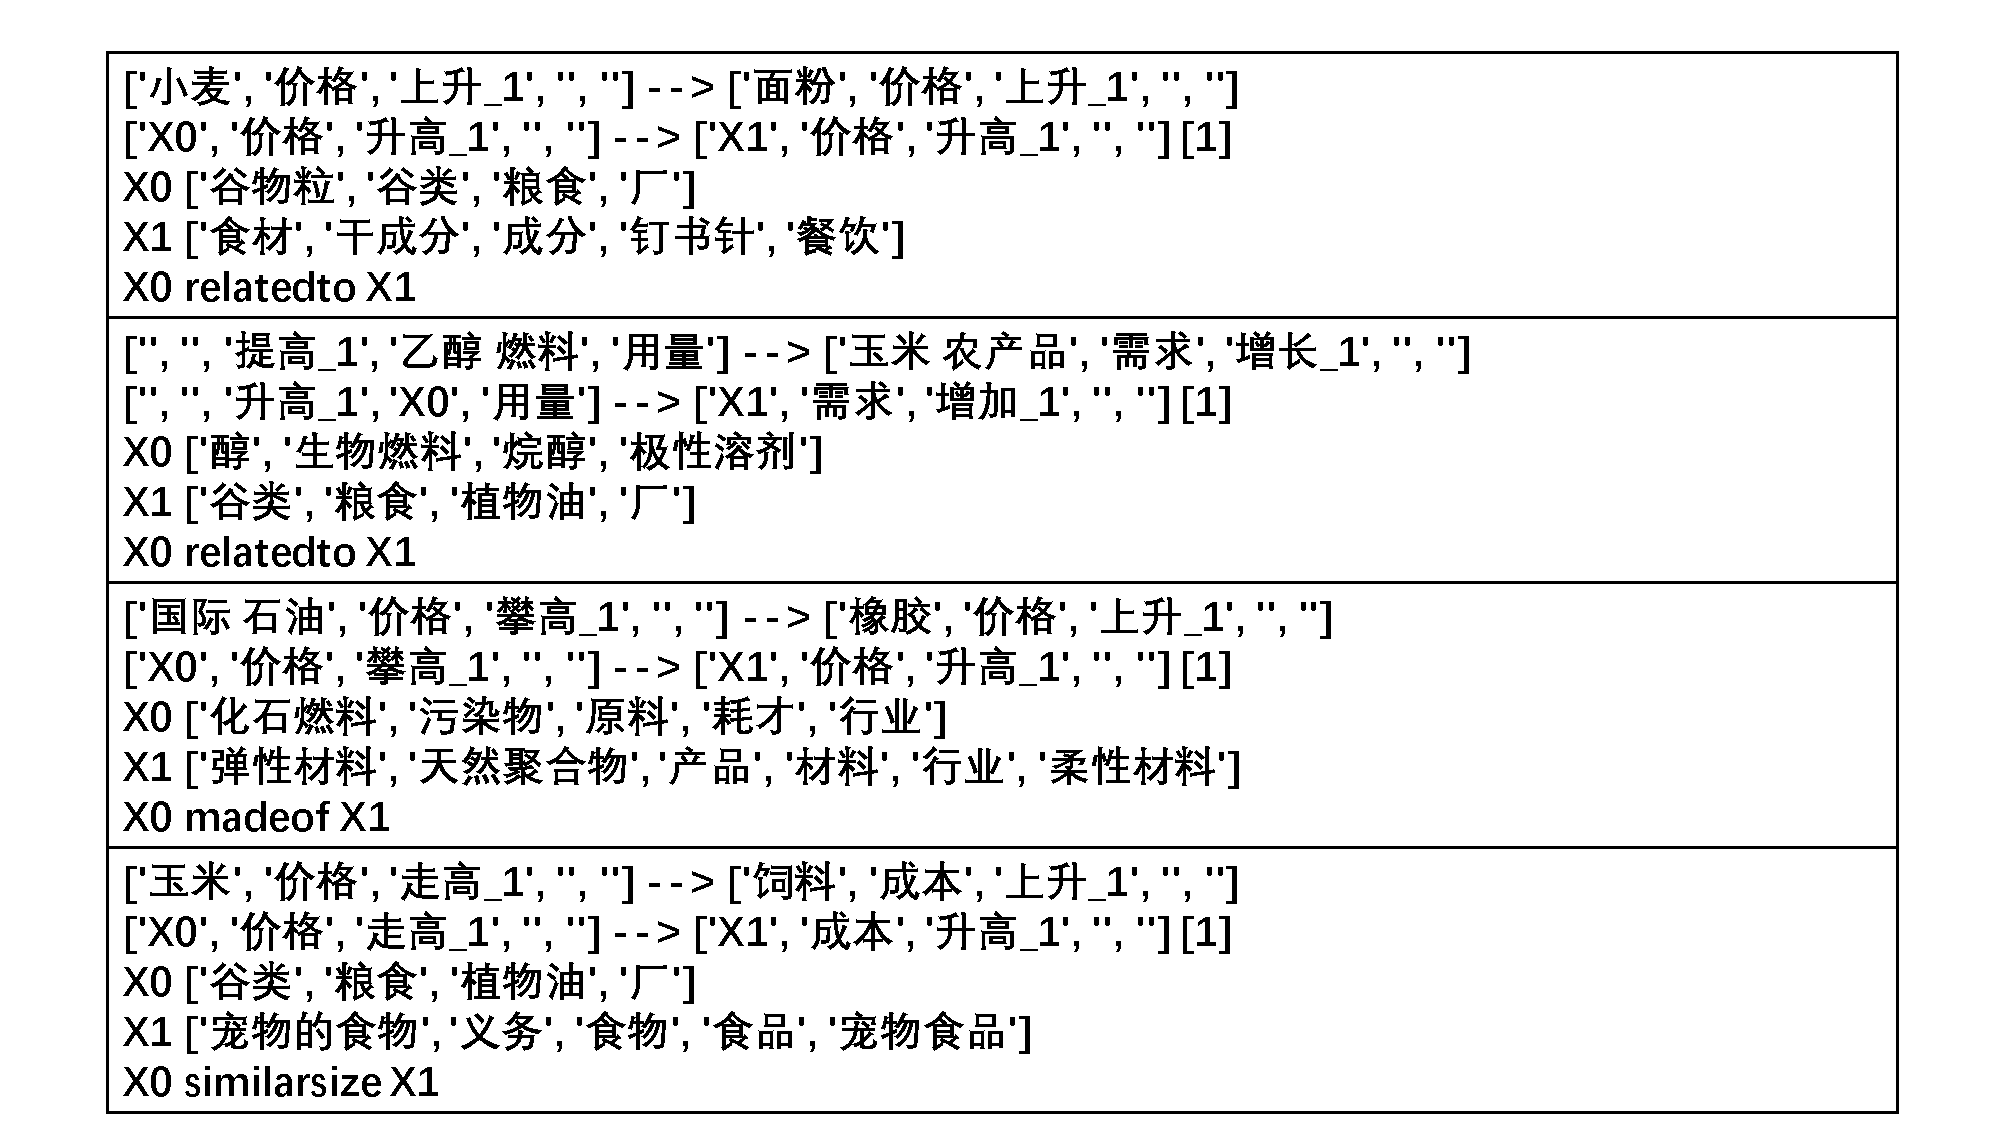
\includegraphics[width=0.9\columnwidth]{figures/good_rule_case}}
	\caption{Good Cases.}
	\label{fig:good_rule_case}
\end{figure}	
	TODO: explanation   
	
\subsubsection{Bad Cases}
\begin{figure}[htbp]
	\centerline{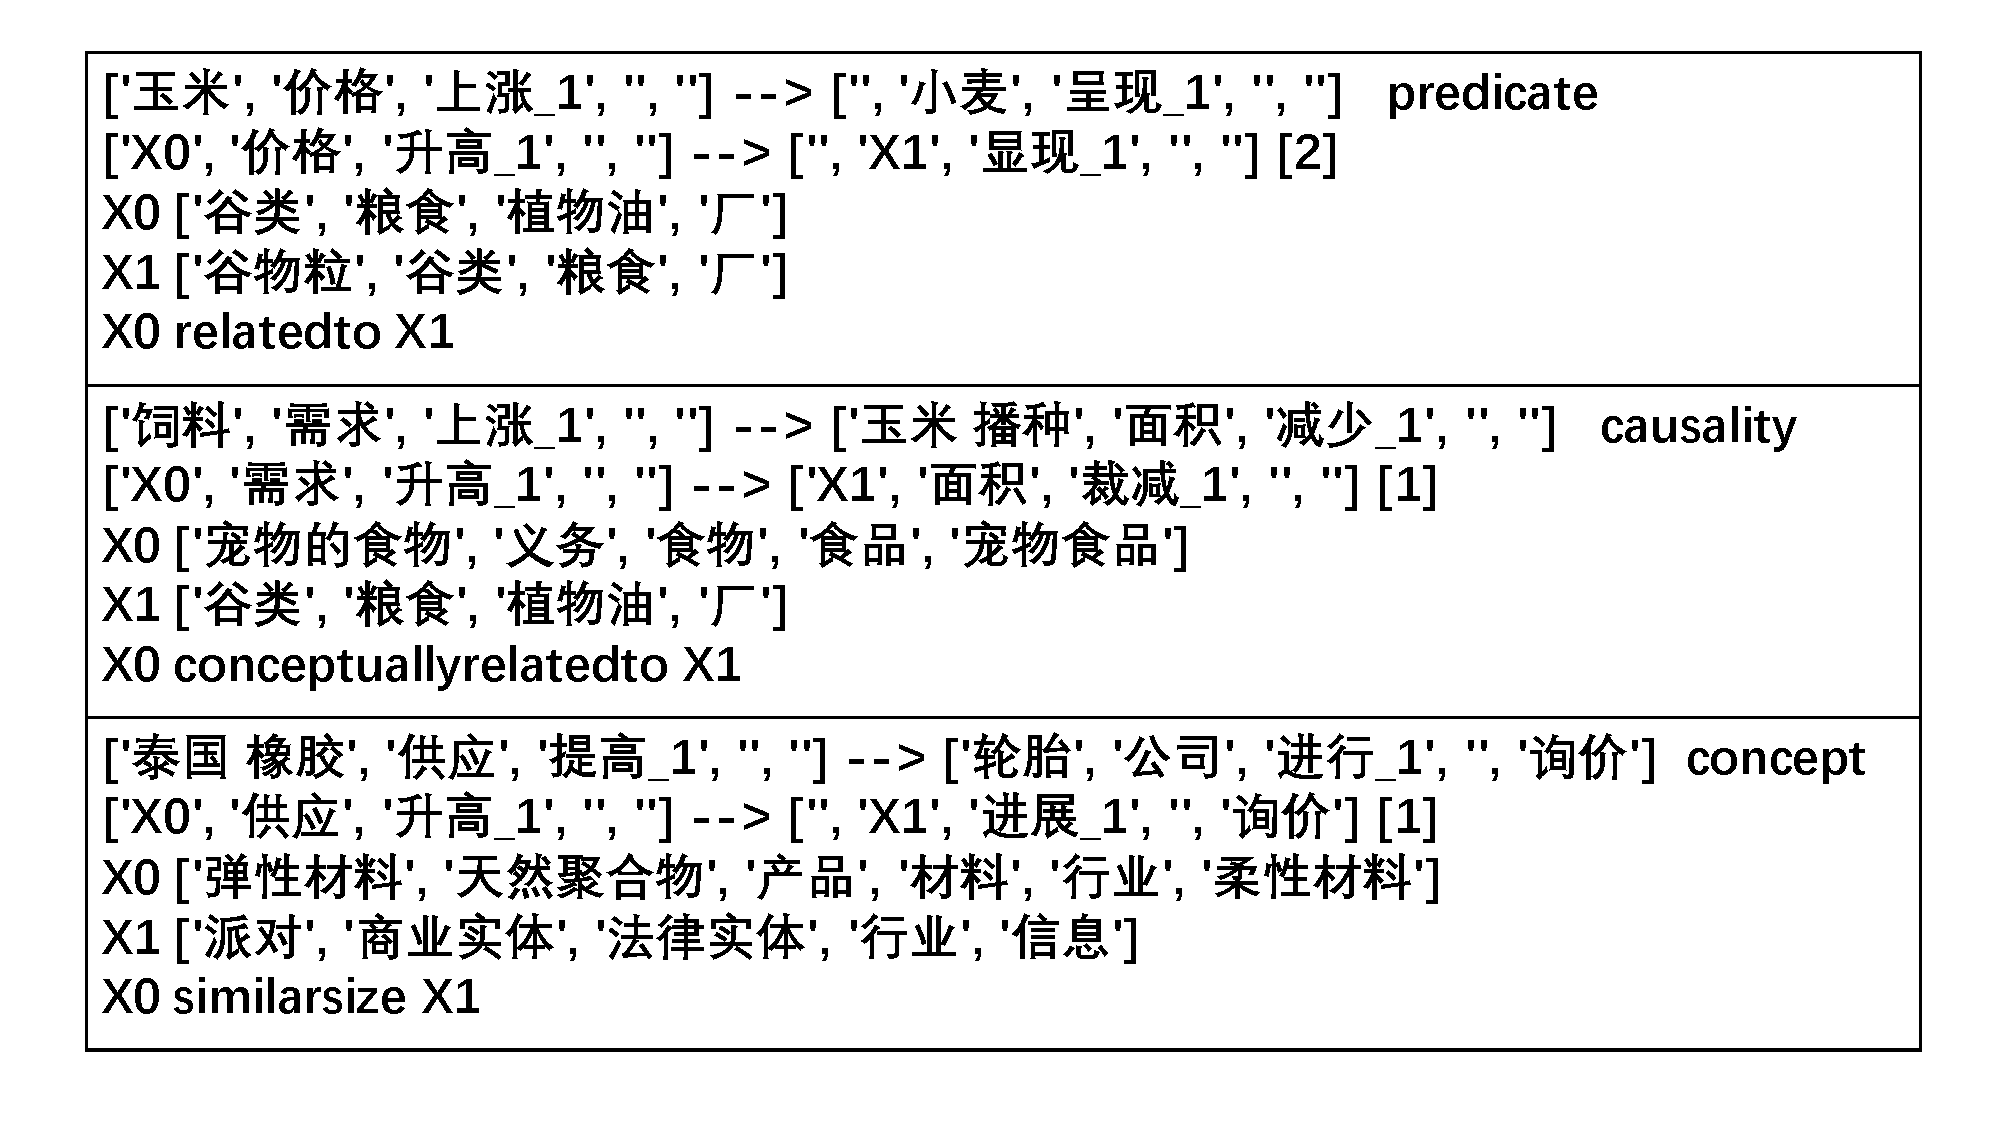
\includegraphics[width=0.9\columnwidth]{figures/bad_rule_case}}
	\caption{Bad Cases.}
	\label{fig:bad_rule_case}

\end{figure}
	TODO: explanation why they are bad
	




\subsection{Rule instantiation}
Rule instantiation also called Rule deduction is shown in \ref{fig:instantiation}
\begin{figure}[htbp]
	\centerline{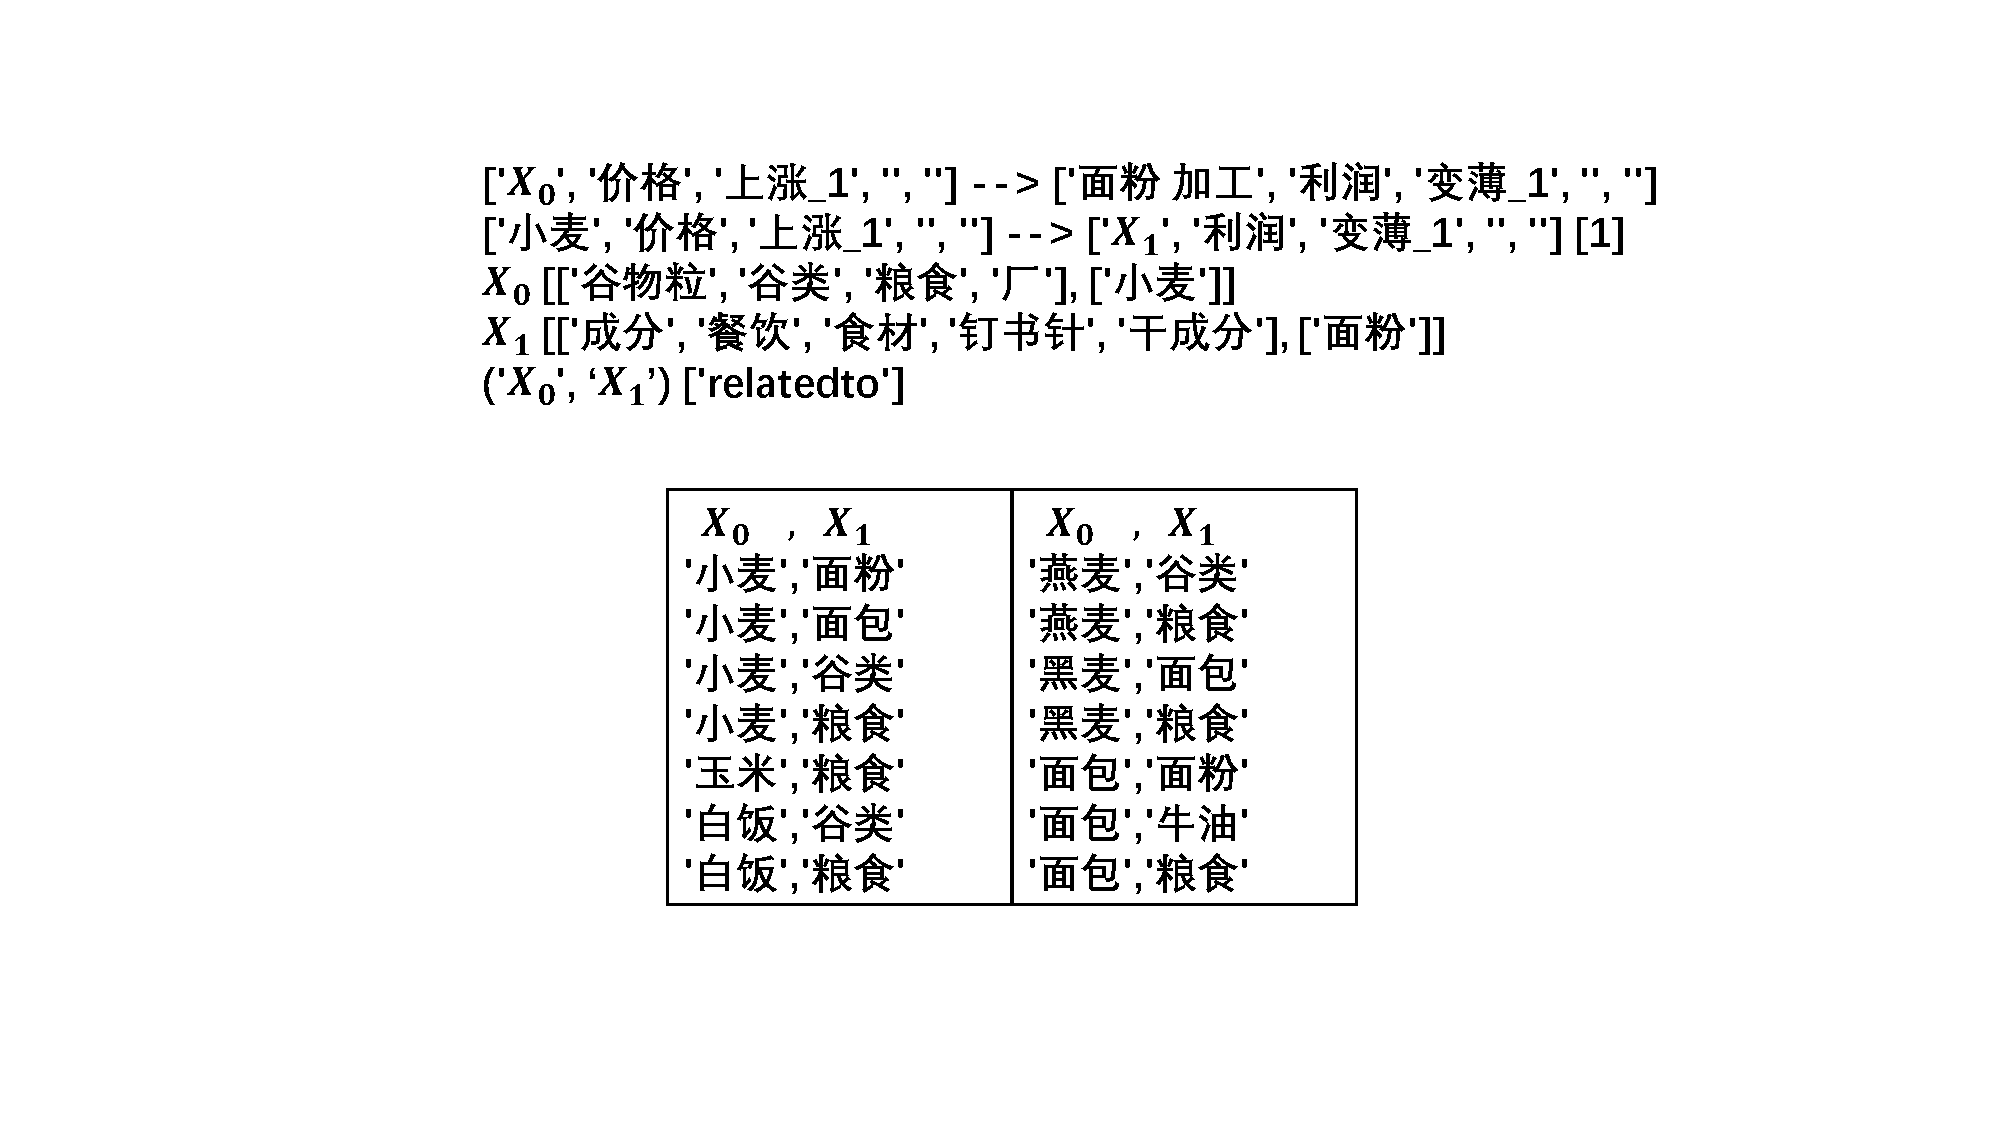
\includegraphics[width=0.9\columnwidth]{figures/instantiation}}
	\caption{Rule Instantiation .}
	\label{fig:instantiation}
\end{figure}

%\textit{Question Answer}
%\textit{Make decision}






